\documentclass[10pt]{beamer}

\usetheme[background=dark, numbering=fraction]{metropolis}
\usepackage{appendixnumberbeamer}
\usepackage{color, xcolor}
\usepackage{dsfont}
\definecolor{mydarkblue}{rgb}{0,0.08,0.45}


\usepackage{booktabs}
\usepackage[scale=2]{ccicons}


\usepackage{adjustbox} 
\usepackage{pgfplots}
\usepgfplotslibrary{dateplot}
\usepackage{fourier-orns}
\usepackage{xspace}
\usepackage{tikz}
\usetikzlibrary{scopes,matrix,positioning}
\tikzset{
  mymx/.style={matrix of math nodes,nodes=myball,column sep=4em,row sep=-1ex},
  myball/.style={draw,circle,inner sep=0pt},
  mylabel/.style={midway,sloped,fill=white,inner sep=1pt,outer sep=1pt,below,
    execute at begin node={$\scriptstyle},execute at end node={$}},
  plain/.style={draw=none,fill=none},
  sel/.append style={fill=green!10},
  prevsel/.append style={fill=red!10},
  route/.style={-latex,thick},
  selroute/.style={route,blue!50!green}
}

\usepackage[backend=bibtex,style=authoryear]{biblatex}
\addbibresource{index.bib}
\renewcommand*{\bibfont}{\scriptsize}



\newcommand{\themename}{\textbf{\textsc{metropolis}}\xspace}
\DeclareMathOperator*{\argmin}{arg\,min}
\DeclareMathOperator*{\minimize}{minimize}
\DeclareMathOperator*{\maximize}{maximize}

\makeatletter
\renewcommand{\metropolis@colors@dark}{%
  \setbeamercolor{normal text}{%
    fg=black!2,
    bg=mDarkTeal
  }%
  \usebeamercolor[fg]{normal text}%
}
\renewcommand{\metropolis@colors@light}{%
  \setbeamercolor{normal text}{%
    fg=mDarkTeal,
    bg=black!2
  }%
  \usebeamercolor[fg]{normal text}%
}
\makeatother

\title{\huge Parallel Optimization and Machine Learning}
\author{
\large{\bfseries Fabian Pedregosa}}
% {\normalsize{ includes work with Remi Leblond and Simon Lacoste-Julien}}}
% \author{
% \hspace{4.8em}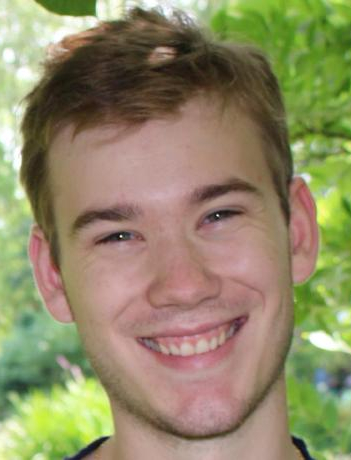
\includegraphics[width=0.2\linewidth]{img/remi}
% \hspace{4.8em}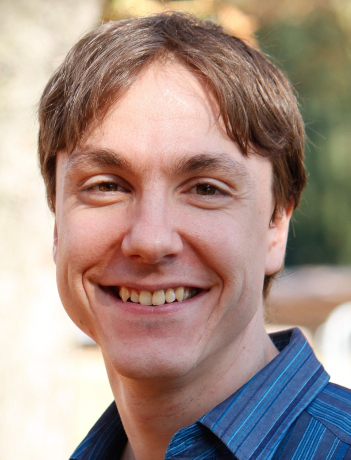
\includegraphics[width=0.2\linewidth]{img/SLJ}
% }\\
% {\normalsize\vphantom{}\hspace{0.5em} Fabian Pedregosa \hspace{3.5em} R\'emi Leblond \hspace{2.2em} Simon Lacoste--Julien}\\
% \vphantom{}\\
% \vphantom{}
\includegraphics[width=0.3\linewidth]{img/logo_inria}
% 
\includegraphics[width=0.12\linewidth]{img/ens.png}
% \hspace{0.5em}
\includegraphics[width=0.3\linewidth]{img/montreal}
% \hspace{0.5em}
\includegraphics[width=0.2\linewidth]{img/mila}
% }
% 
\institute{

{\centerline{\hspace{2em}
\includegraphics[width=0.3\linewidth]{img/Berkeley_wordmark_gold_no_uc}\hspace*{2em}

\includegraphics[width=0.3\linewidth]{img/eth_logo_kurz_neg}\hspace*{2em}
{
\includegraphics[width=0.25\linewidth]{img/eu}}
}}
}
%\titlegraphic{\hfill\includegraphics[height=1.5cm]{figures/UCBerkeley_wordmark_blue.eps}}
\date{\vspace{1em}\today~{Huawei Paris Research Center}}

\begin{document}

\maketitle

\metroset{background=light} % change background theme according to manual
{
\usebackgroundtemplate{%
\begin{picture}(40,260)
  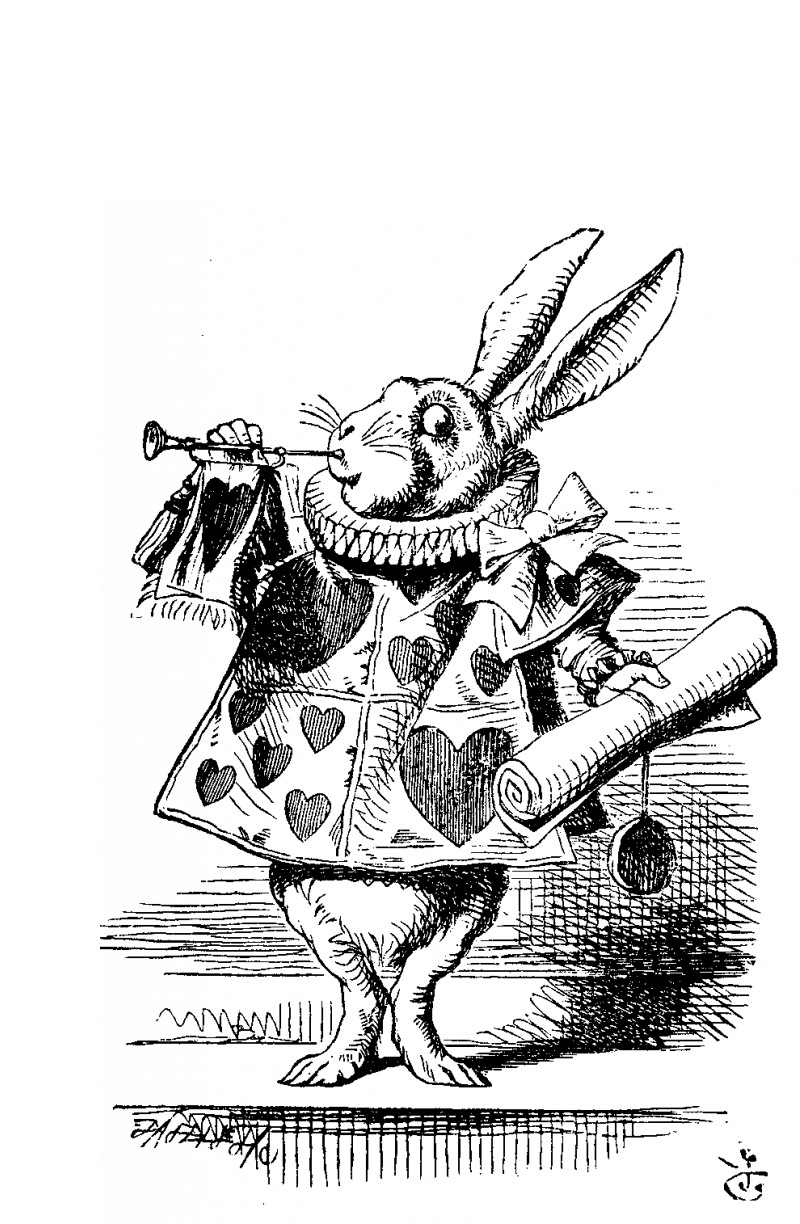
\includegraphics[height=0.9\paperheight]{img/white-rabbit}
  \end{picture}
  }
\begin{frame}{About me}
\begin{columns}
\begin{column}{0.4\textwidth}  %%<--- here
\end{column}
\begin{column}{0.6\textwidth}  %%<--- here
\begin{itemize}
\item Engineer (2010-2012), Inria Saclay.
\item PhD (2012-2015, Inria Saclay)
\item Postdoc (2015-2016), Dauphine--ENS--Inria Paris.
\item Postdoc (2017-present), UC Berkeley - ETH Zurich (Marie-Curie fellowship, European Commission)
\end{itemize}
\end{column}
\end{columns}
\end{frame}
}

\metroset{background=dark} % change background theme according to manual

\begin{frame}{Motivation}
\begin{columns}[T] % align columns
\begin{column}{.5\textwidth}
\centering{Computer add in 1993}
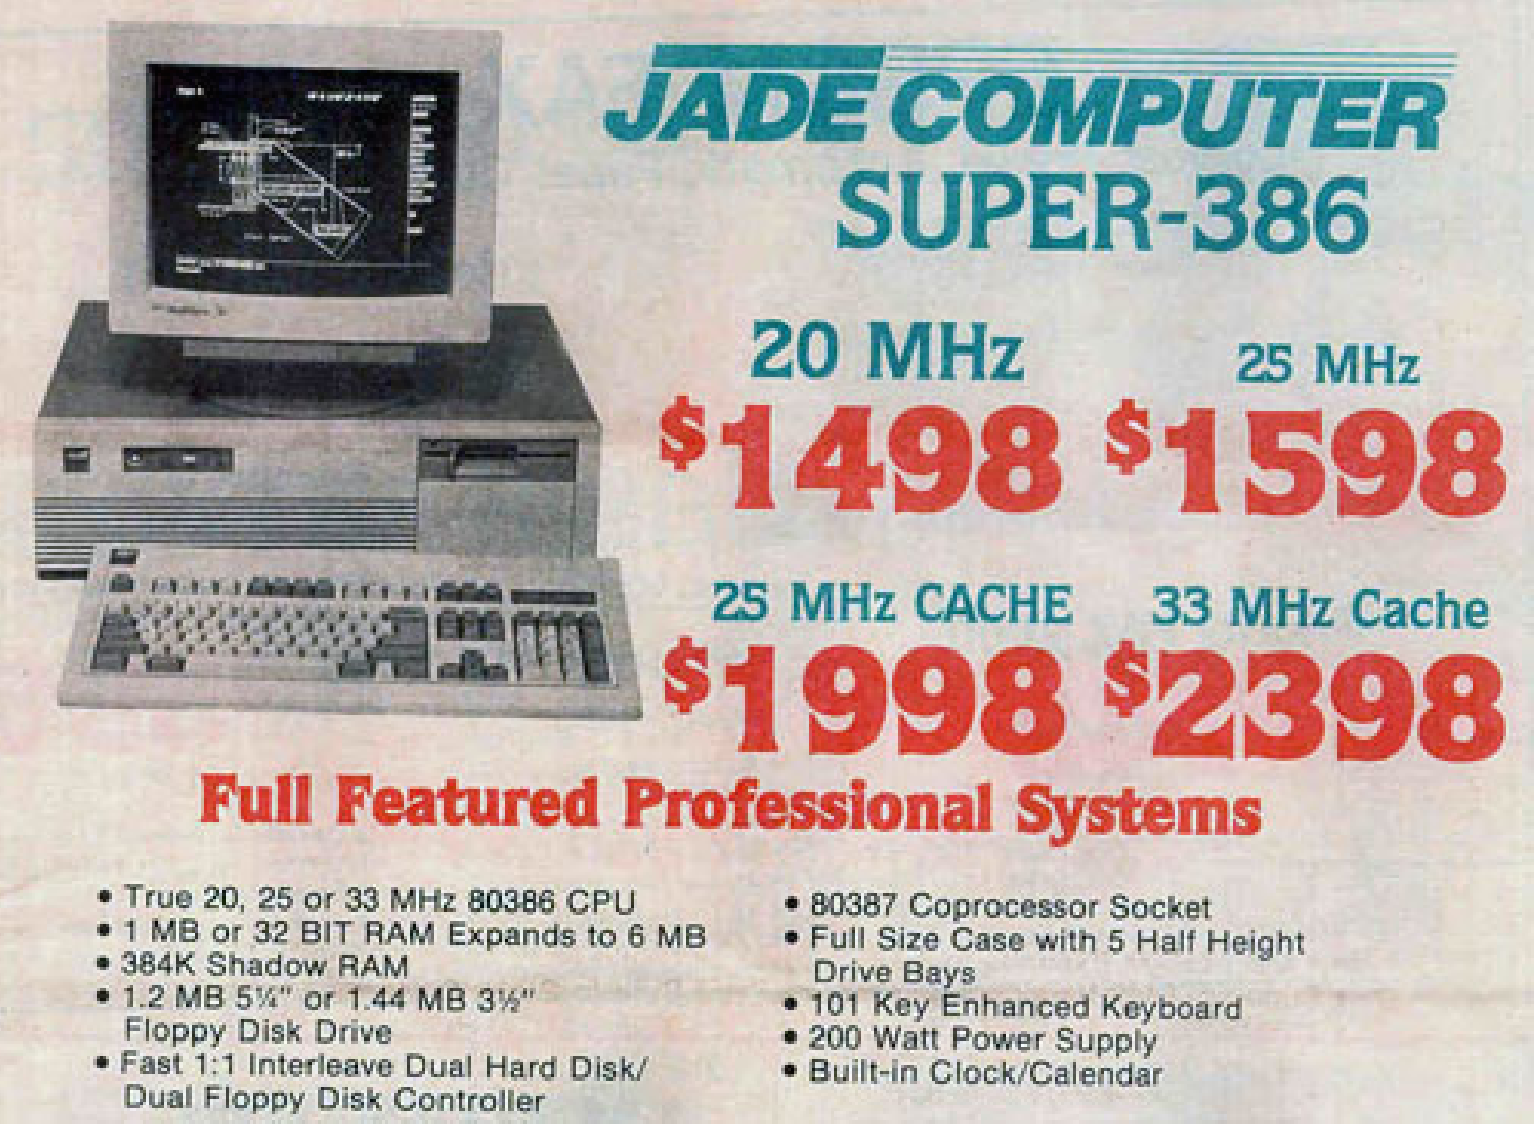
\includegraphics[width=1.05\linewidth]{img/old_ad}
\end{column}%
\hfill%
\begin{column}{.5\textwidth}
\centering{Computer add in 2006}
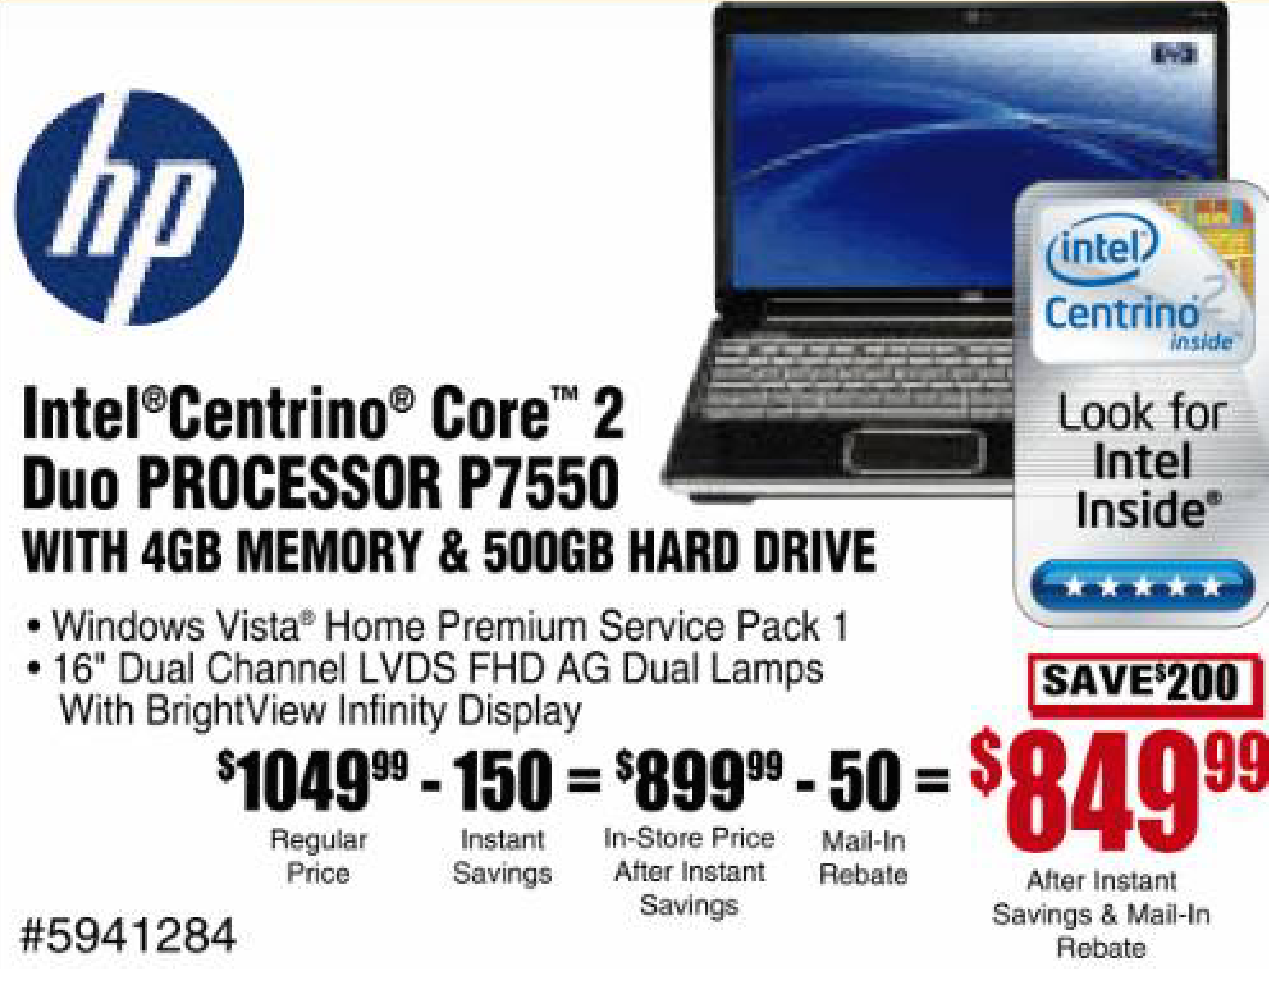
\includegraphics[width=\linewidth]{img/2006_ad}
\end{column}%
\end{columns}
What has changed?
\pause
2006 = no longer mentions to speed of processors
\end{frame}


\begin{frame}{Moore's law}
\begin{quote}
The complexity for minimum component costs 
has increased at a rate of roughly a factor of 
two per year. Certainly over the short term this 
rate can be expected to continue
\end{quote}
Gordon Moore (Intel), 1965

\hspace{1em}\begin{quote}
OK, maybe a factor of two every two 
years.
\end{quote}
Gordon Moore (Intel), 1975 [paraphrased]
\end{frame}


\begin{frame}{40 years of CPU trends}
\centering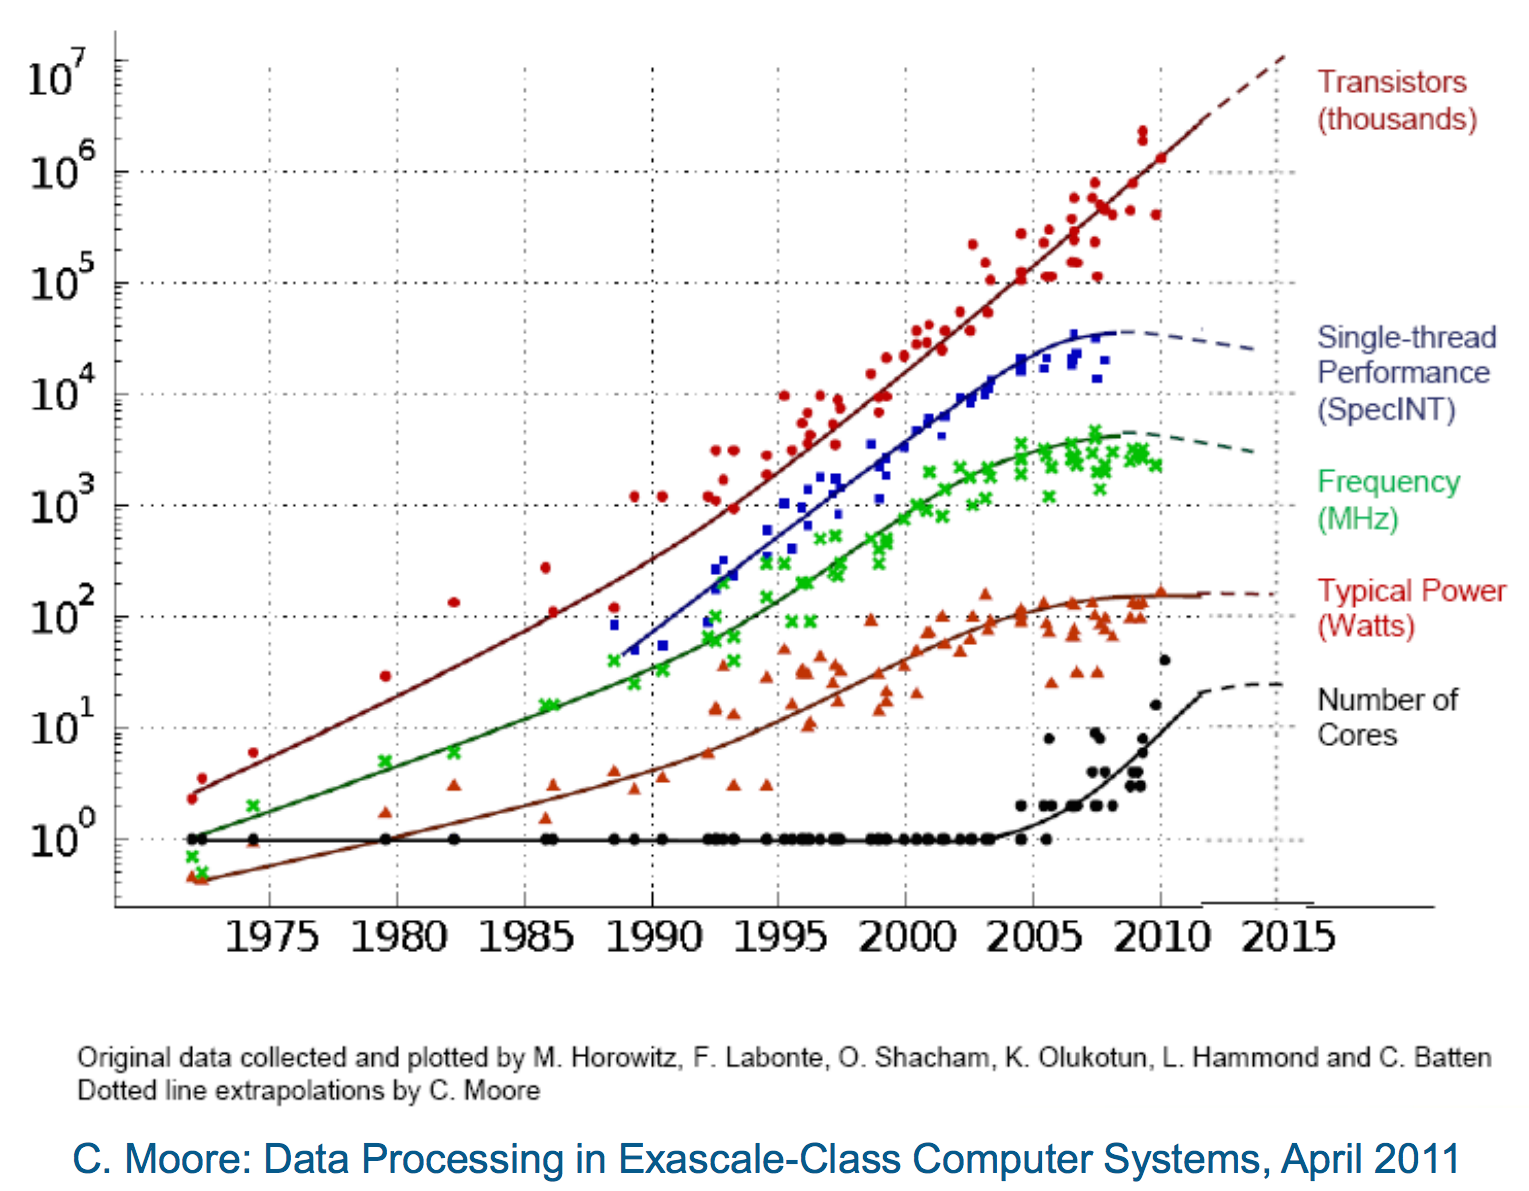
\includegraphics[width=0.8\linewidth]{img/moore_law}

\begin{itemize}[<+->]
\item Speed of CPUs has stagnated since 2005;
\item Multi-core architectures are here to stay.
\end{itemize}
\pause {\bfseries Parallel algorithms needed to take advantage of modern CPUs.}
\end{frame}


\begin{frame}{Outline}

{\bfseries Goal of the talk:} overview and state of the art in parallel optimization methods in machine learning.

\medskip

\begin{columns}[T] % align columns
\begin{column}{.5\textwidth}
{\centering \bfseries Synchronous methods}
\begin{itemize}
\item ADMM
\item MapReduce (and variants: Hadoop, Spark)
\item COCOA
\end{itemize}
\end{column}%
\hfill%
\begin{column}{.5\textwidth}
{\centering \bfseries Asynchronous methods}
\begin{itemize}
\item Asynchronous SGD
\item Variance-reduced methods
\end{itemize}
\end{column}%
\end{columns}
\vspace{1em}

Along the way, analysis of algorithms, our recent work.

\end{frame}

\begin{frame}{Outline}
Parallel algorithms can be divided  large categories: 
synchronous and asynchronous methods.

\begin{figure}
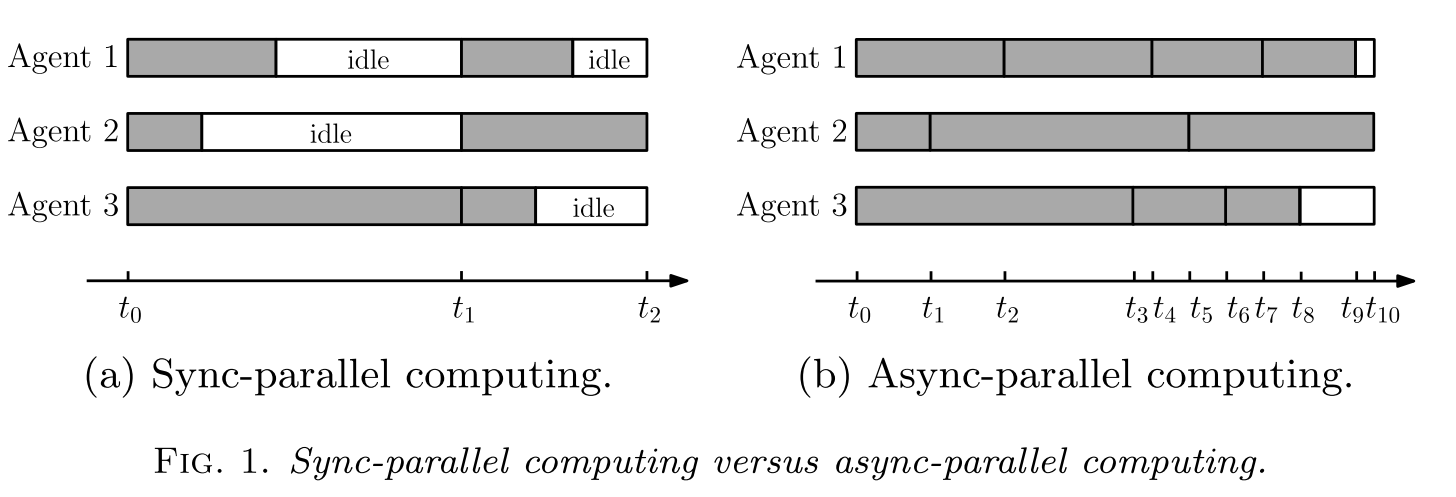
\includegraphics[width=\linewidth]{img/sync_vs_async}
{\small Image credits: \parencite{peng2016arock}}
\end{figure}
\end{frame}


\begin{frame}{The problem}
The kind of parallelization will depend on the problem.

The kind of problem that we will be interested in

The problem: supervised learning.

Common abstraction in optimization: minimize a finite sum
\end{frame}

\begin{frame}{X}

\begin{tikzpicture}
  \matrix[mymx] (mx) {
    &|[prevsel]| f_1(e) \\
    |[plain]| x_1 && f_4(e) \\
    &|[sel]| f_2(e) && f_6(e) & |[plain]| y \\
    |[plain]| x_2 && f_5(e) \\
    & f_3(e) \\
  };
  {[route]
    \foreach \y in {2,4} {
      \draw (mx-\y-1) -- (mx-1-2);
      \draw (mx-\y-1) -- (mx-5-2);
      \draw (mx-\y-3) -- (mx-3-4); }
    \foreach \y in {1,3,5} {
      \draw (mx-\y-2) -- (mx-2-3);
      \draw (mx-\y-2) -- (mx-4-3); }
    \draw (mx-3-4) -- (mx-3-5);
  }
  {[selroute]
    \draw (mx-2-1) -- (mx-3-2) node[mylabel,above] { W_{(x1)2} };
    \draw (mx-4-1) -- (mx-3-2) node[mylabel] { W_{(x2)2} };
  }
  \node[above right=of mx.center]  {$ y_2 = f_2 (w_{(x1)2} x_1 + w_{(x2)2} x_2) $};
\end{tikzpicture}

\end{frame}


\begin{frame}{XXX}
Minimize $F(x) = \frac{1}{n}\sum^{n}_{i=1} f_i(x)$

Gradient descent [Cauchy, 1847]: descend along $-F'(x)$

Updates of the form $$x^+ = x - \gamma F'(x)$$
Stochastic gradient descent (SGD) [Robbins and Monro, 1951]: select a random index $i$ and descent along $~f_i'(x)$,


Updates of the form $$x^+ = x - \gamma^k f_i'(x)$$
Images source: Francis Bach

\end{frame}



% 
% \begin{frame}[fragile]{Generalization}
% This approach can be naturally generalized to $K$ classes.
% \begin{align}
% \Pr(Y_i=1) &= \frac{e^{\boldsymbol\beta_1 \cdot \mathbf{X}_i}}{1 + \sum_{k=1}^{K-1} e^{\boldsymbol\beta_k \cdot \mathbf{X}_i}} \nonumber \\
% \Pr(Y_i=2) &= \frac{e^{\boldsymbol\beta_2 \cdot \mathbf{X}_i}}{1 + \sum_{k=1}^{K-1} e^{\boldsymbol\beta_k \cdot \mathbf{X}_i}} \\
% \cdots & \cdots \\
% \Pr(Y_i=K-1) &= \frac{e^{\boldsymbol\beta_{K-1} \cdot \mathbf{X}_i}}{1 + \sum_{k=1}^{K-1} e^{\boldsymbol\beta_k \cdot \mathbf{X}_i}}
% \end{align}
% \end{frame}
% 
% 
% \begin{frame}[fragile]{Application}
% Lets use this to predict the future!
% 
% \pause
% Use the data from the religion dataset to predict how religious beliefs will evolve after 2017
% 
% \includegraphics[width=0.5\linewidth]{figures/religion.png}
% 
% \pause
% Suggestion: use scikit-learn's LogisticRegression class with {multi\_class='multinomial'}. Use as features the year and cohort. The model can predict probabilities with method predict\_proba.
% 
% \end{frame}
% 
% 
% 
% \begin{frame}[fragile]{Application}
% 
% 
% To predict, use the same data but with year and cohort shifted accordingly.
% 
% \includegraphics[width=0.5\linewidth]{figures/logistic_future.png}
% 
% 
% 
% \end{frame}
% 
% 
% 
\begin{frame}[noframenumbering, allowframebreaks]
\nocite{pedregosa2017proxasaga}
  % \frametitle{References}
  \printbibliography
 \end{frame}

\end{document}
